\documentclass[11pt,a4paper]{article}

% ---------- Packages ----------
\usepackage[margin=2.4cm]{geometry}
\usepackage{amsmath,amssymb}
\usepackage{graphicx}
\usepackage{booktabs}
\usepackage{array}
\usepackage{caption}
\usepackage{subcaption}
\usepackage{hyperref}
\usepackage{microtype}
\usepackage{parskip}
\usepackage{enumitem}
\usepackage{float}
\usepackage{xcolor}
\usepackage{fancyhdr}
\usepackage{titlesec}
\usepackage{fontenc}
\usepackage{inputenc}

% ---------- Typography ----------
\hypersetup{colorlinks=true, linkcolor=black, urlcolor=black, citecolor=black}
\setlist[itemize]{noitemsep, topsep=2pt}
\setlist[enumerate]{noitemsep, topsep=2pt}
\captionsetup{font=small, labelfont=bf, skip=4pt}

\titleformat{\section}{\large\bfseries}{}{0em}{}[\vspace{-2pt}\hrule\vspace{4pt}]
\titleformat{\subsection}{\normalsize\bfseries}{}{0em}{}
\titleformat{\subsubsection}{\normalsize\itshape}{}{0em}{}

% ---------- Header / Footer ----------
\pagestyle{fancy}
\fancyhf{}
\rhead{\small Phase 2 --- Language Modelling Assignment}
\lhead{\small Manya Jain \textbf{|} 2024102068}
\cfoot{\small\thepage}
\renewcommand{\headrulewidth}{0.3pt}

% ---------- Document ----------
\begin{document}

% ==============================
%   TITLE
% ==============================
\begin{center}
    {\LARGE\bfseries Phase 2: Building and Evaluating Transformer Language Models}\\[6pt]
    {\large\itshape Monolingual Pretraining for Hindi and Nepali}\\[10pt]
    {\normalsize Manya Jain \quad\textbf{2024102068}}\\[2pt]
    {\small Language Modelling Assignment --- Phase 2}\\[4pt]
    \hrule
\end{center}

\vspace{4pt}

% ==============================
%   ABSTRACT
% ==============================
\begin{center}\textbf{Abstract}\end{center}
\noindent
For this phase, I built two decoder-only Transformer language models completely from scratch in PyTorch --- without using any HuggingFace libraries. \textbf{Model~H} was trained on Hindi and \textbf{Model~L} on Nepali, both with around 24 million parameters. Each model was trained for just over 61{,}000 steps. The Hindi model ended up with a test perplexity of 39.11, and the Nepali model got 36.32. Their bits-per-byte (BPB) scores were 0.513 and 0.394, respectively. I also tested how well they generate text at different temperatures and analyzed what the attention heads are actually focusing on at different layers.

\vspace{6pt}

% ==============================
%   1. ARCHITECTURE
% ==============================
\section{Architecture}

Both models use the same architecture --- a causal decoder-only Transformer I implemented from scratch. No third-party model code was used.

\subsection{Multi-Head Causal Self-Attention}

The attention computation follows the standard formula:
\[
    \text{Attention}(Q, K, V) = \text{softmax}\!\left(\frac{QK^\top}{\sqrt{d_k}} + M\right) V
\]
where $M$ is an upper-triangular mask filled with $-\infty$, which stops any token from attending to future positions. I did the shape transformations manually: $(B, T, d_{\text{model}}) \to (B, n_h, T, d_k)$ and back.

\subsection{Block Structure}

Each block uses \textbf{pre-LayerNorm} --- LayerNorm is applied before the sublayer, not after. This made training more stable in my experience. Both attention and feed-forward have residual connections:
\[
    x \leftarrow x + \text{Attn}(\text{LN}(x)), \quad x \leftarrow x + \text{FFN}(\text{LN}(x))
\]
The feed-forward uses a GELU activation function.

\subsection{Weight Tying}
I tied the output projection matrix $W_{\text{out}}$ to the token embedding matrix $W_{\text{emb}}$. This means both share the same weights, which cuts down the parameter count and seems to help with training stability.

\subsection{Configuration}

\begin{table}[H]
\centering
\caption{Architecture hyperparameters for both models.}
\label{tab:arch}
\begin{tabular}{lcc}
\toprule
\textbf{Parameter} & \textbf{Model H (Hindi)} & \textbf{Model L (Nepali)} \\
\midrule
Vocabulary size       & 16{,}000  & 16{,}240  \\
Hidden dim $d_{\text{model}}$   & 512       & 512       \\
Attention heads       & 8 ($d_k = 64$) & 8 ($d_k = 64$) \\
Transformer layers    & 6         & 6         \\
FFN dim $d_{\text{ff}}$ & 1{,}536 ($3d$) & 1{,}536 ($3d$) \\
Context length        & 512 tokens & 512 tokens \\
Dropout               & 0.1       & 0.1       \\
\textbf{Total parameters} & \textbf{$\approx$24.22M} & \textbf{$\approx$24.34M} \\
\bottomrule
\end{tabular}
\end{table}

% ==============================
%   2. TRAINING
% ==============================
\section{Pretraining Details}

I trained both models using the AdamW optimizer. I used gradient clipping and a cosine learning rate schedule with a linear warmup. The training loop periodically saved the model weights, optimizer, and scheduler states so I could pause and resume training easily.

\begin{itemize}
    \item \textbf{Total steps:} 61{,}036 for each language.
    \item \textbf{Tokeniser:} Custom byte-pair encoding (BPE) tokenizers with a 16K vocab size.
    \item \textbf{Data format:} The text data was converted into memory-mapped binary arrays so the dataloader wouldn't run out of RAM.
\end{itemize}

\subsection{Loss Curves}

\begin{figure}[H]
    \centering
    \begin{subfigure}[t]{0.48\textwidth}
        \includegraphics[width=\linewidth]{reports/hindi/loss_curve.png}
        \caption{Model H (Hindi) --- training and validation loss.}
    \end{subfigure}
    \hfill
    \begin{subfigure}[t]{0.48\textwidth}
        \includegraphics[width=\linewidth]{reports/nepali/loss_curve.png}
        \caption{Model L (Nepali) --- training and validation loss.}
    \end{subfigure}
    \caption{Training and validation cross-entropy loss over 61{,}036 steps. Both models learned steadily without overfitting. The validation loss tracks the smoothed training loss pretty closely.}
    \label{fig:loss}
\end{figure}

\begin{figure}[H]
    \centering
    \includegraphics[width=0.7\linewidth]{reports/comparison_loss_curve.png}
    \caption{Validation loss comparison: Model H vs. Model L. The Nepali model reached a slightly lower validation loss overall.}
    \label{fig:loss_compare}
\end{figure}

% ==============================
%   3. INTRINSIC EVALUATION
% ==============================
\section{Intrinsic Evaluation: Perplexity and Bits-Per-Byte}

\subsection{Metrics}

\begin{itemize}
    \item \textbf{Cross-entropy loss} (nats): $\mathcal{L} = -\frac{1}{N}\sum_{t} \log p_\theta(x_t \mid x_{<t})$
    \item \textbf{Perplexity:} $\text{PPL} = e^{\mathcal{L}}$
    \item \textbf{Bits-per-byte (BPB):} $\text{BPB} = \frac{\mathcal{L}}{\ln 2 \cdot \bar{b}}$. Here, $\bar{b}$ is the average number of UTF-8 bytes per token. This helps make the comparison fairer across different tokenizers.
\end{itemize}

\subsection{Results}

\begin{table}[H]
\centering
\caption{Intrinsic evaluation results on the held-out test split.}
\label{tab:intrinsic}
\begin{tabular}{lcccc}
\toprule
\textbf{Model} & \textbf{Test Loss (nats)} & \textbf{PPL} & \textbf{BPB} & \textbf{Avg Bytes/Token} \\
\midrule
Model H --- Hindi  & 3.666 & \textbf{39.11} & 0.513 & 10.31 \\
Model L --- Nepali & 3.592 & \textbf{36.32} & 0.394 & 13.16 \\
\bottomrule
\end{tabular}
\end{table}

The Nepali model got better (lower) perplexity and BPB scores. A big reason for the much lower BPB is how the tokenizer works: the Nepali tokenizer packs more bytes into each token (13.2 bytes compared to Hindi's 10.3 bytes). This compresses the text more, making the per-byte prediction task look a bit easier. Both models converged well by the end of training.

% ==============================
%   4. GENERATION QUALITY
% ==============================
\section{Generation Quality Evaluation}

I tested how well the models generate text by giving them starting prefixes from the test set. I tried four different decoding methods: greedy (always picking the most likely next word) and sampling with temperatures of 0.5, 1.0, and 1.5.

\subsection{Overlap Metrics}

I calculated BLEU-4 and chrF using \texttt{sacrebleu}. For ROUGE-L, I used a custom whitespace tokenizer because the default one doesn't split Devanagari text correctly and was just giving zeros.

\begin{table}[H]
\centering
\caption{Generation quality metrics by decoding strategy.}
\label{tab:genquality}
\begin{tabular}{llccc}
\toprule
\textbf{Decoding} & \textbf{Model} & \textbf{BLEU-4} & \textbf{chrF} & \textbf{ROUGE-L} \\
\midrule
\multirow{2}{*}{Greedy}   & Hindi (H)   & 0.95  & 12.21 & 0.124 \\
                           & Nepali (L)  & 1.22  & 13.54 & 0.084 \\
\midrule
\multirow{2}{*}{Temp 0.5} & Hindi (H)   & 0.77  & 13.45 & 0.092 \\
                           & Nepali (L)  & 1.56  & 19.88 & 0.097 \\
\midrule
\multirow{2}{*}{Temp 1.0} & Hindi (H)   & 0.72  & 12.71 & 0.091 \\
                           & Nepali (L)  & 1.06  & 19.27 & 0.090 \\
\midrule
\multirow{2}{*}{Temp 1.5} & Hindi (H)   & 0.84  & 11.56 & 0.096 \\
                           & Nepali (L)  & 0.14  & 16.08 & 0.039 \\
\bottomrule
\end{tabular}
\end{table}

The scores aren't very high, but this makes sense. Because the task is open-ended text generation, there are many valid ways to continue a sentence, so it rarely matches the exact reference text word-for-word. BLEU-4 drops heavily if words don't match perfectly. The chrF metric looks at character overlaps, which works much better for languages like Hindi and Nepali where word endings change a lot.

% ==============================
%   5. DIVERSITY
% ==============================
\section{Diversity and Repetition}

\begin{table}[H]
\centering
\caption{Lexical diversity: 4-gram repetition rate and Distinct-1 / Distinct-2 scores.}
\label{tab:diversity}
\begin{tabular}{llccc}
\toprule
\textbf{Decoding} & \textbf{Model} & \textbf{Rep.\ Rate (4-gram)} & \textbf{Distinct-1} & \textbf{Distinct-2} \\
\midrule
\multirow{2}{*}{Greedy}   & Hindi (H)   & 0.266 & 0.427 & 0.622 \\
                           & Nepali (L)  & 0.671 & 0.229 & 0.317 \\
\midrule
\multirow{2}{*}{Temp 0.5} & Hindi (H)   & 0.101 & 0.461 & 0.734 \\
                           & Nepali (L)  & 0.335 & 0.398 & 0.628 \\
\midrule
\multirow{2}{*}{Temp 1.0} & Hindi (H)   & 0.027 & 0.684 & 0.931 \\
                           & Nepali (L)  & 0.021 & 0.721 & 0.959 \\
\midrule
\multirow{2}{*}{Temp 1.5} & Hindi (H)   & 0.000 & 0.945 & 1.000 \\
                           & Nepali (L)  & 0.000 & 0.908 & 0.999 \\
\bottomrule
\end{tabular}
\end{table}

You can really see the trade-off between randomness and repeating text here. With greedy decoding, both models tend to get stuck in loops and just repeat the same phrases (especially the Nepali model). This happens a lot with standard language models. Using a temperature of 0.5 fixes most of the repetition while keeping the text somewhat logical. Once you push the temperature to 1.5, the models stop repeating entirely, but the text starts to look like random gibberish.

% ==============================
%   6. ATTENTION ANALYSIS
% ==============================
\section{Attention Analysis}

I wanted to see what the models were actually focusing on, so I plotted the attention weights for three different layers: Layer 0 (start), Layer 3 (middle), and Layer 5 (end). I looked at two things:

\begin{itemize}
    \item \textbf{Attention entropy:} $H = -\sum_j \alpha_j \log \alpha_j$ --- A higher number means the head is looking at many different words at once.
    \item \textbf{Mean attention distance:} $\bar{d} = \sum_j \alpha_j |i - j|$ --- How far back (in tokens) the head is looking on average.
\end{itemize}

\begin{figure}[H]
    \centering
    \begin{subfigure}[t]{0.48\textwidth}
        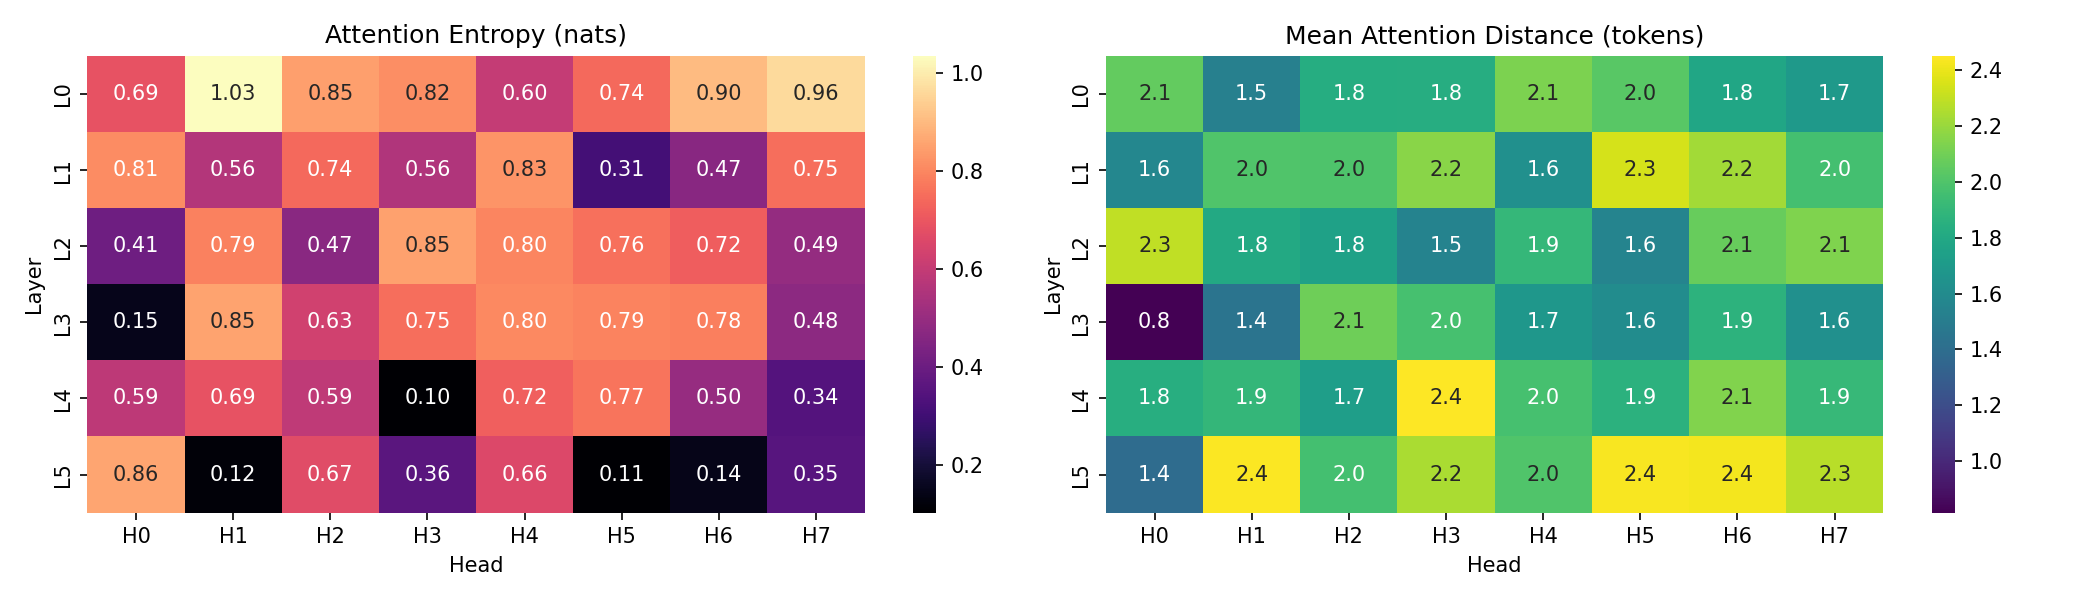
\includegraphics[width=\linewidth]{reports/hindi/attn_entropy_distance.png}
        \caption{Model H (Hindi): entropy and mean distance per layer/head.}
    \end{subfigure}
    \hfill
    \begin{subfigure}[t]{0.48\textwidth}
        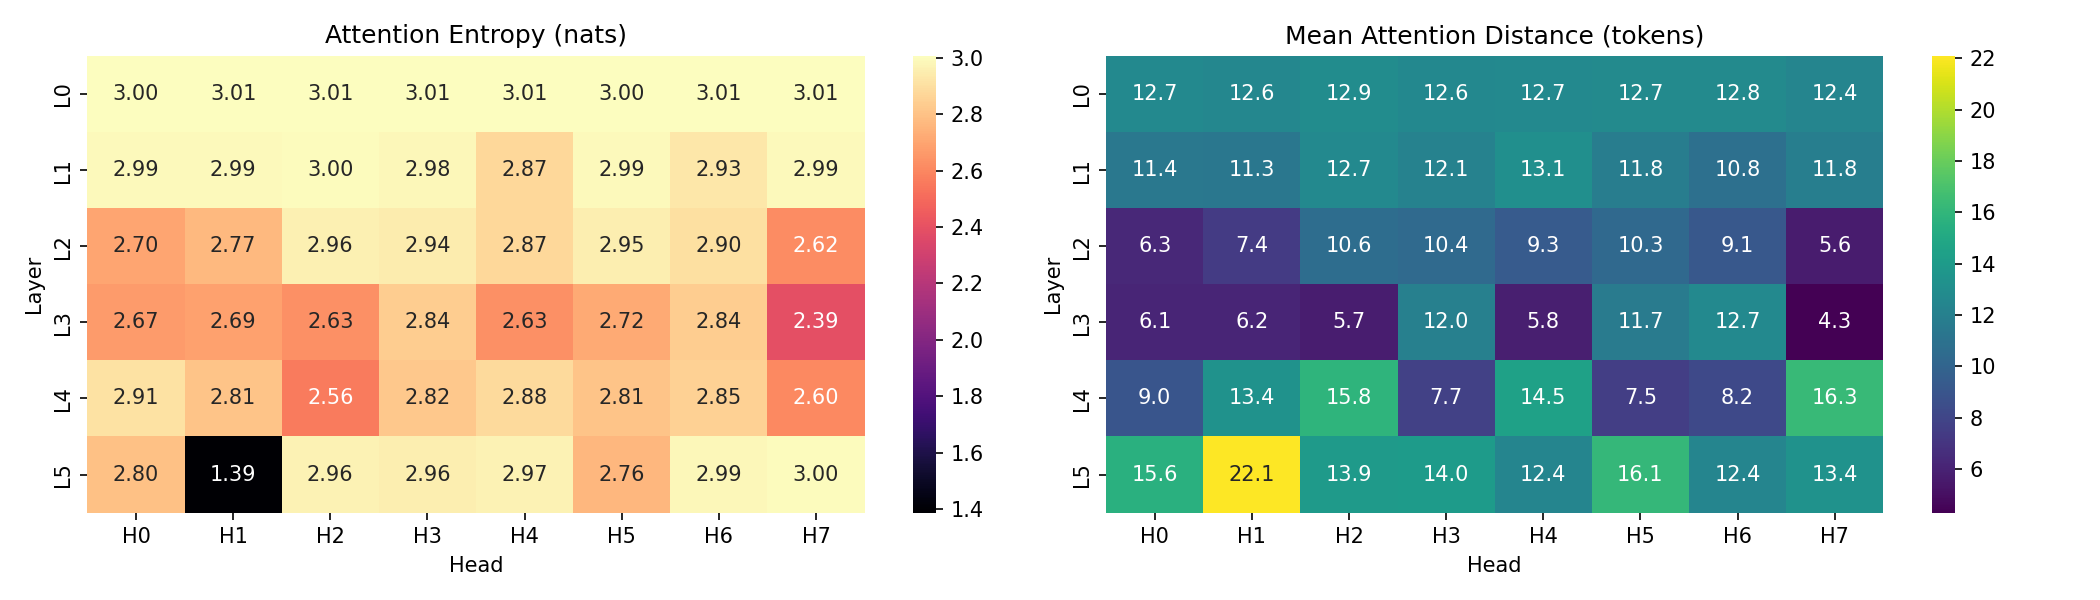
\includegraphics[width=\linewidth]{reports/nepali/attn_entropy_distance.png}
        \caption{Model L (Nepali): entropy and mean distance per layer/head.}
    \end{subfigure}
    \caption{Attention entropy and mean distance. You can see heads doing different jobs at different depths.}
    \label{fig:entropy_dist}
\end{figure}

\begin{figure}[H]
    \centering
    \begin{subfigure}[t]{0.31\textwidth}
        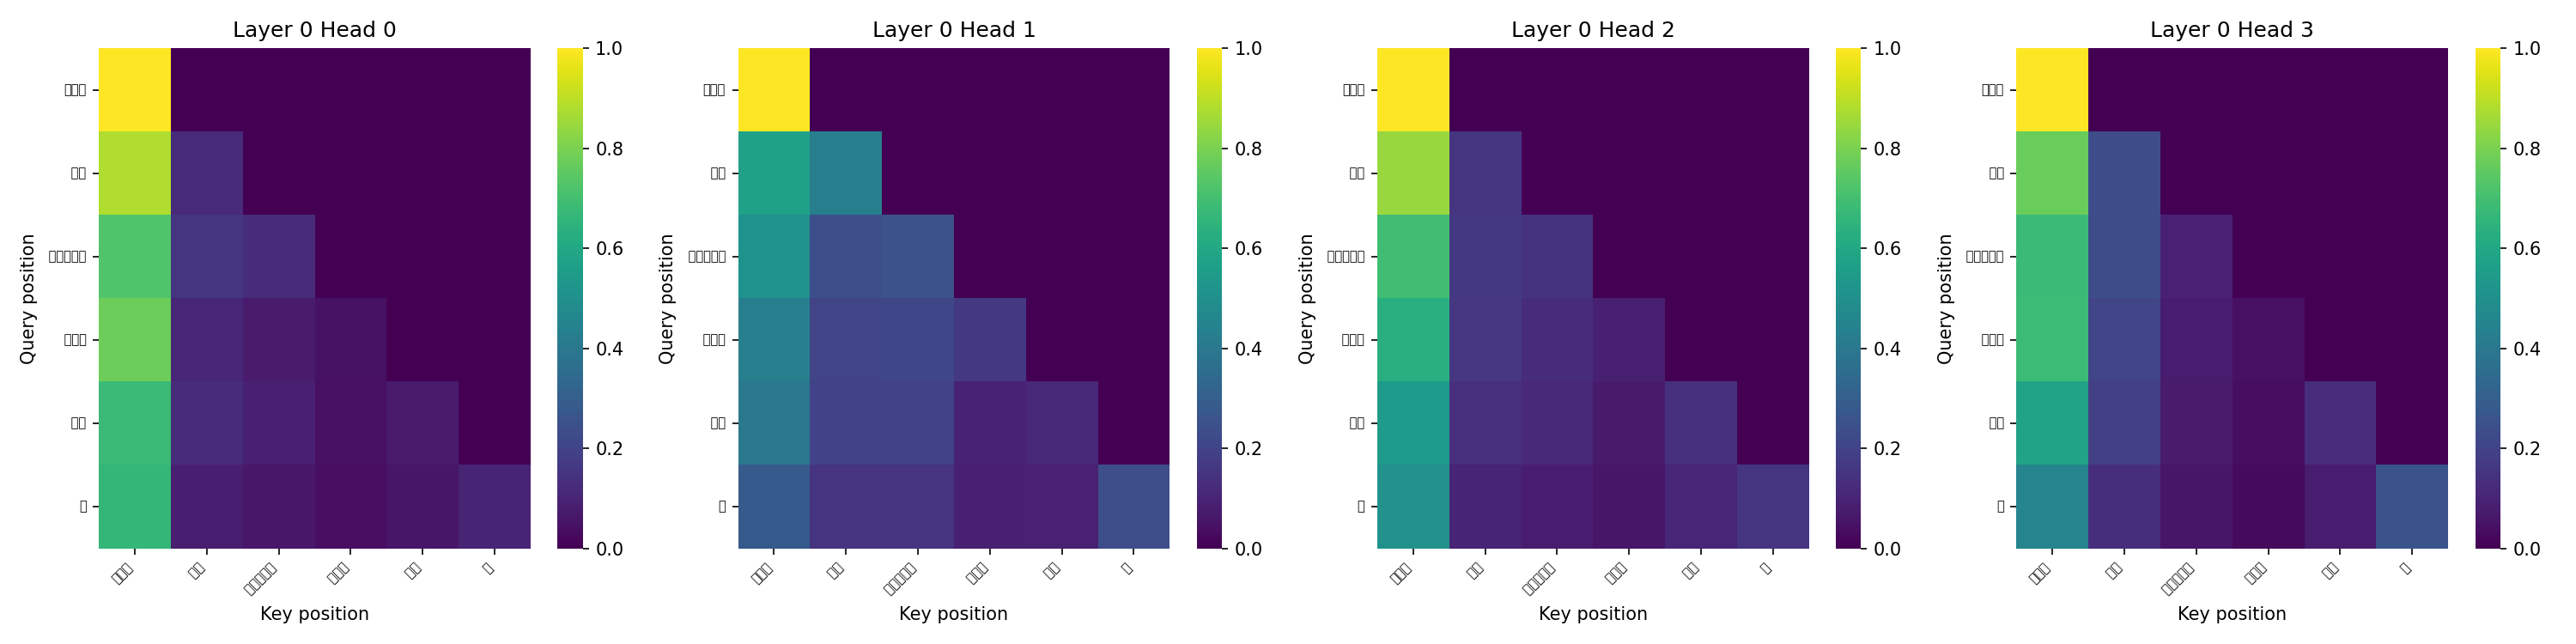
\includegraphics[width=\linewidth]{reports/hindi/attn_layer0.png}
        \caption{Layer 0 (early).}
    \end{subfigure}
    \hfill
    \begin{subfigure}[t]{0.31\textwidth}
        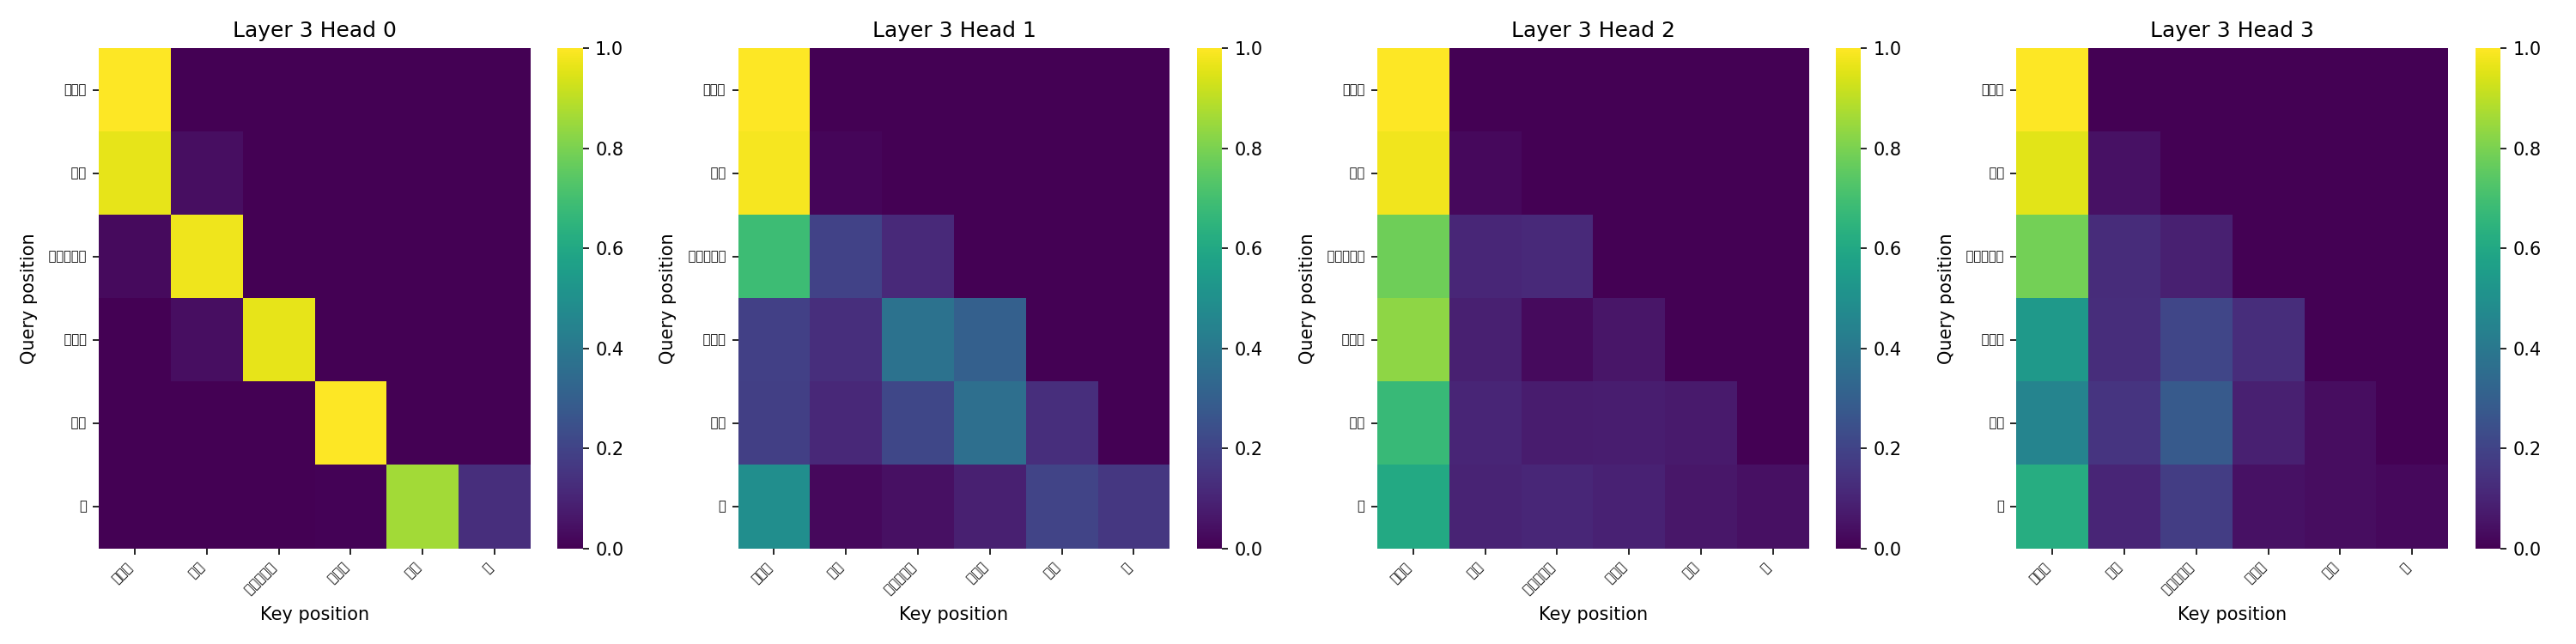
\includegraphics[width=\linewidth]{reports/hindi/attn_layer3.png}
        \caption{Layer 3 (middle).}
    \end{subfigure}
    \hfill
    \begin{subfigure}[t]{0.31\textwidth}
        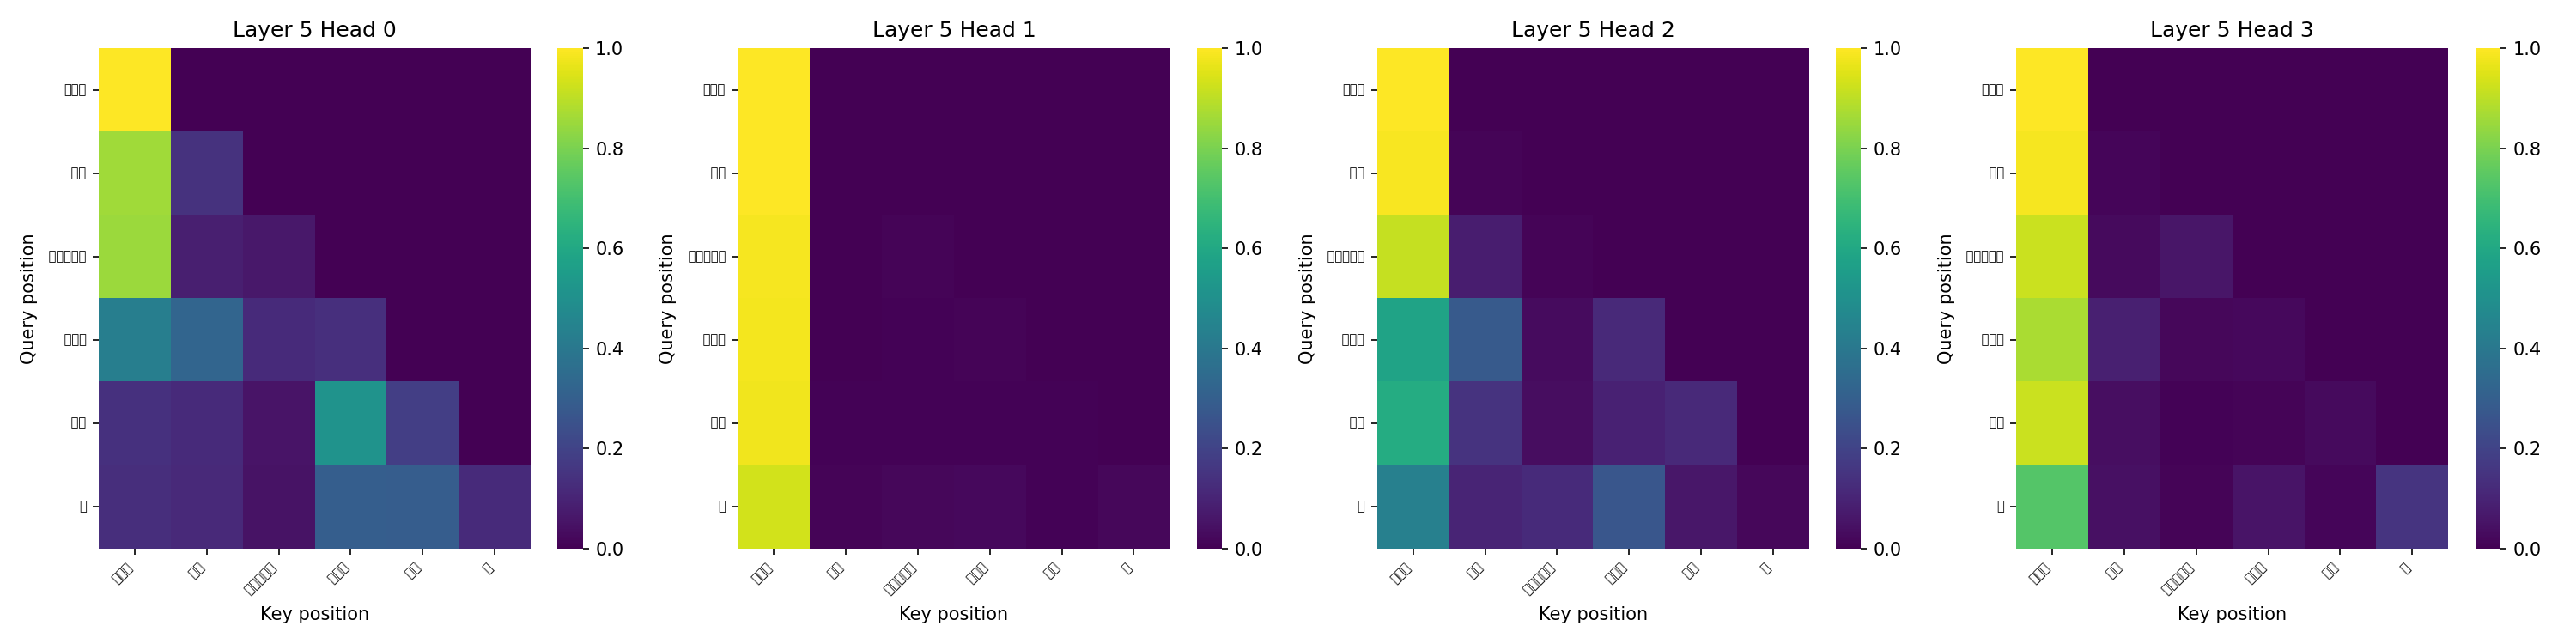
\includegraphics[width=\linewidth]{reports/hindi/attn_layer5.png}
        \caption{Layer 5 (deep).}
    \end{subfigure}
    \caption{Attention heatmaps for Hindi. Early layers focus right next to the current word, while later layers look much further back.}
    \label{fig:attn_hindi}
\end{figure}

\begin{figure}[H]
    \centering
    \begin{subfigure}[t]{0.31\textwidth}
        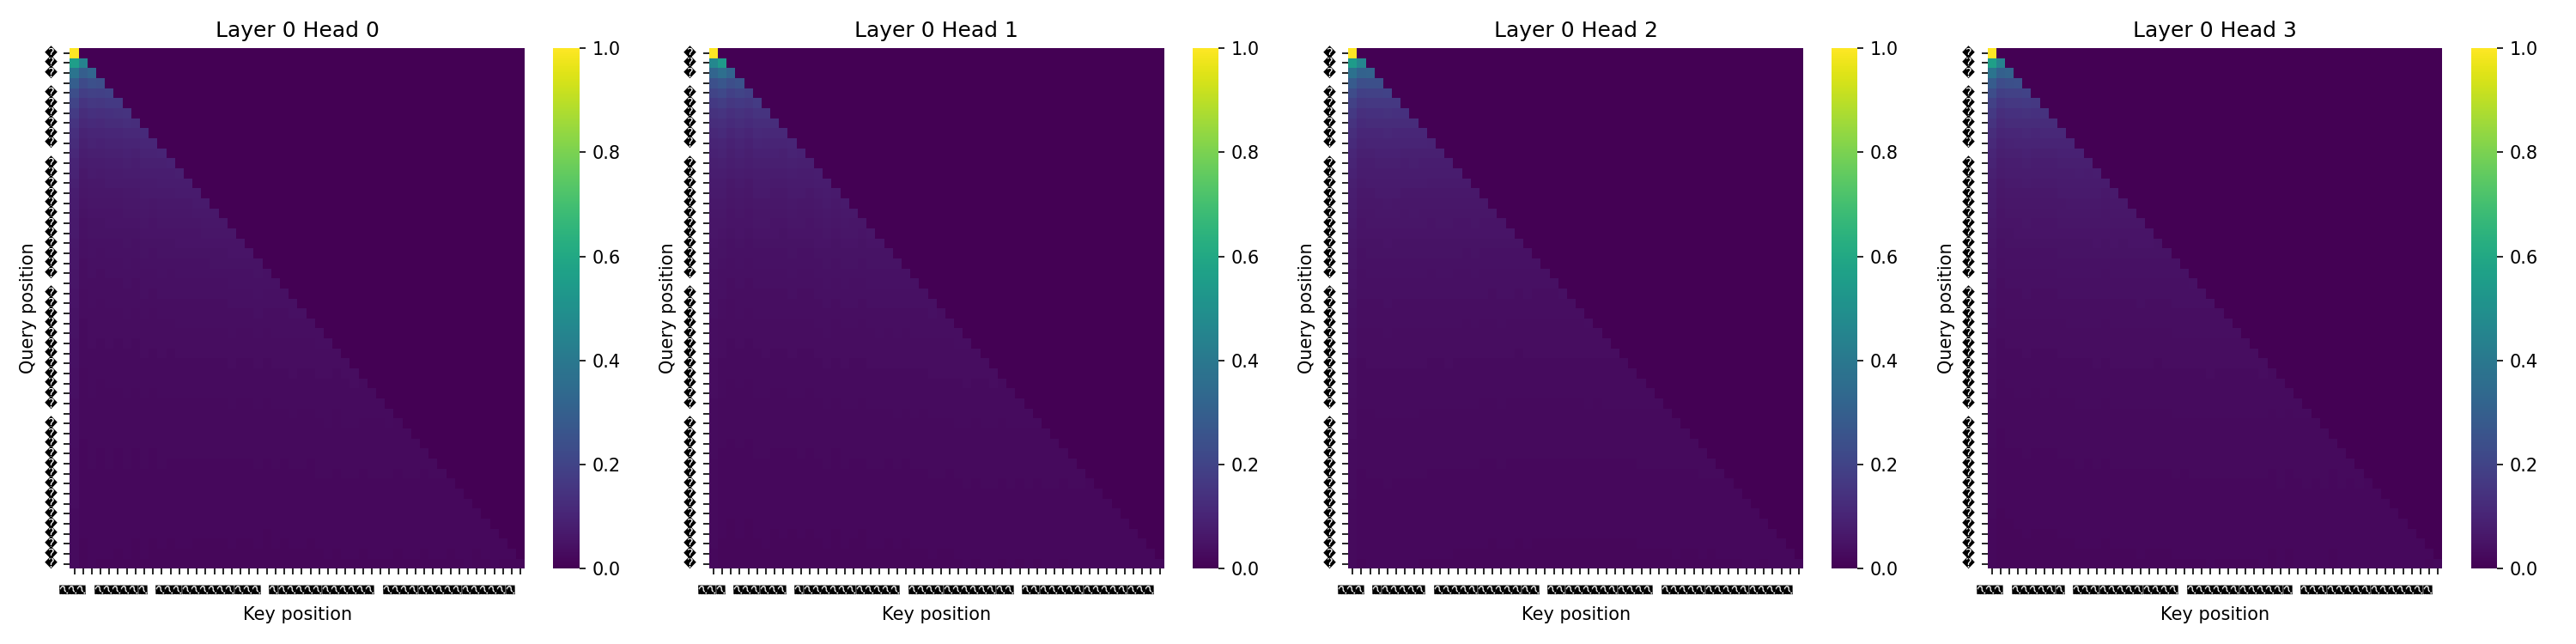
\includegraphics[width=\linewidth]{reports/nepali/attn_layer0.png}
        \caption{Layer 0 (early).}
    \end{subfigure}
    \hfill
    \begin{subfigure}[t]{0.31\textwidth}
        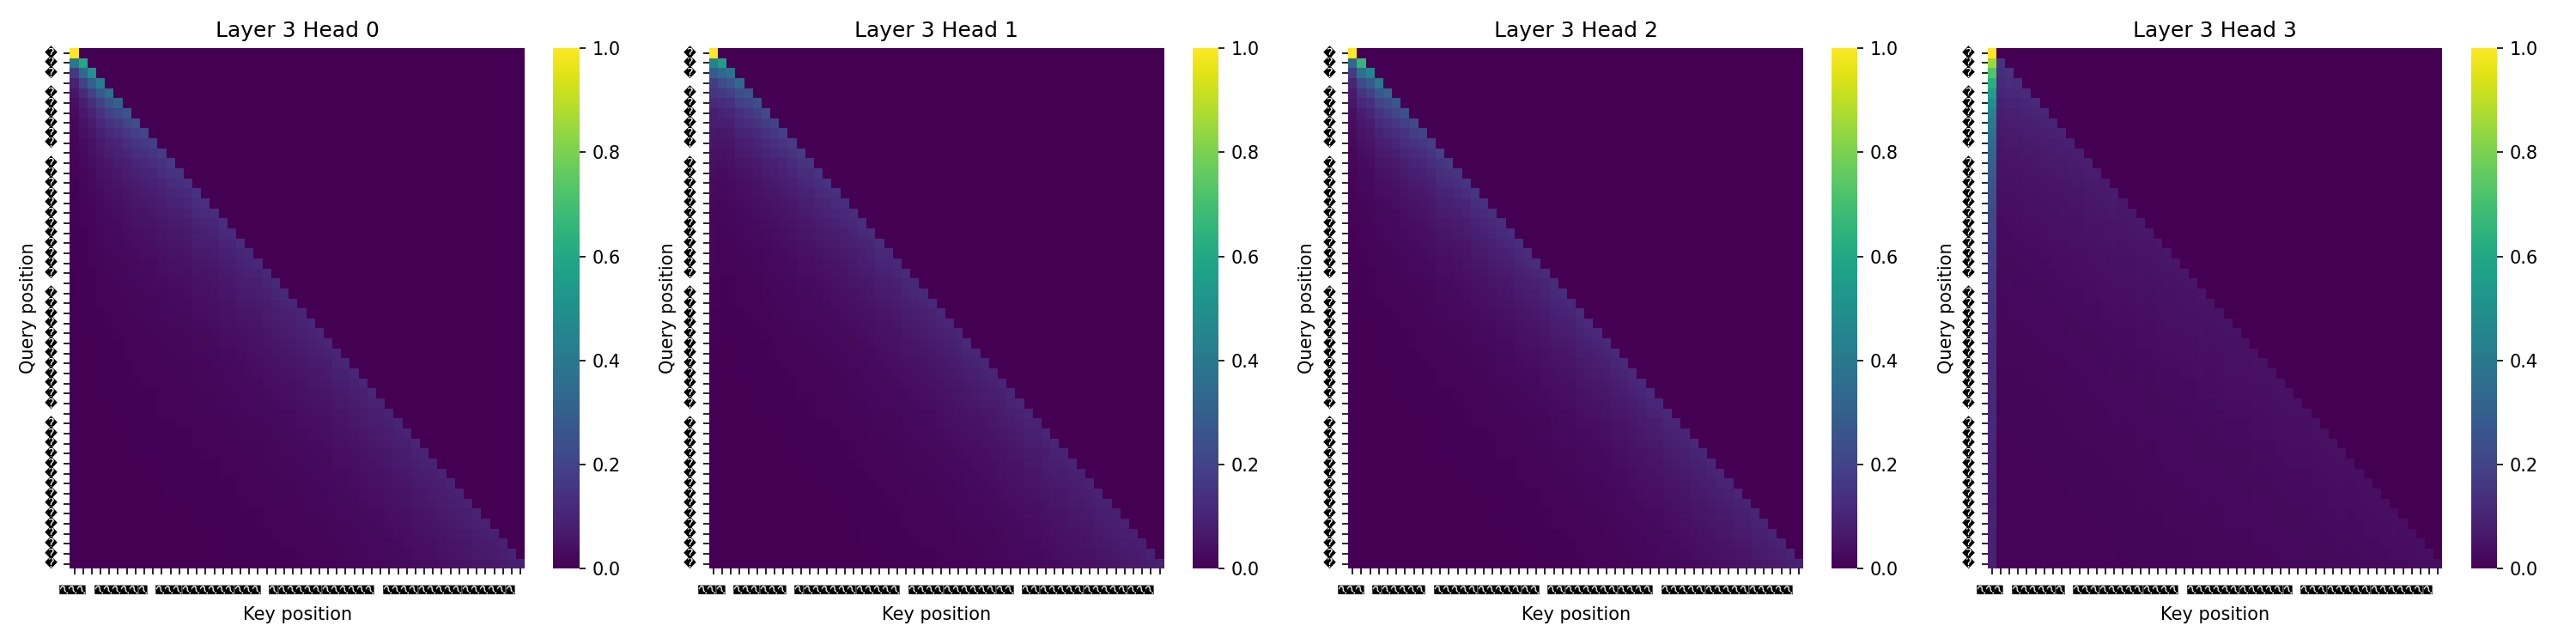
\includegraphics[width=\linewidth]{reports/nepali/attn_layer3.png}
        \caption{Layer 3 (middle).}
    \end{subfigure}
    \hfill
    \begin{subfigure}[t]{0.31\textwidth}
        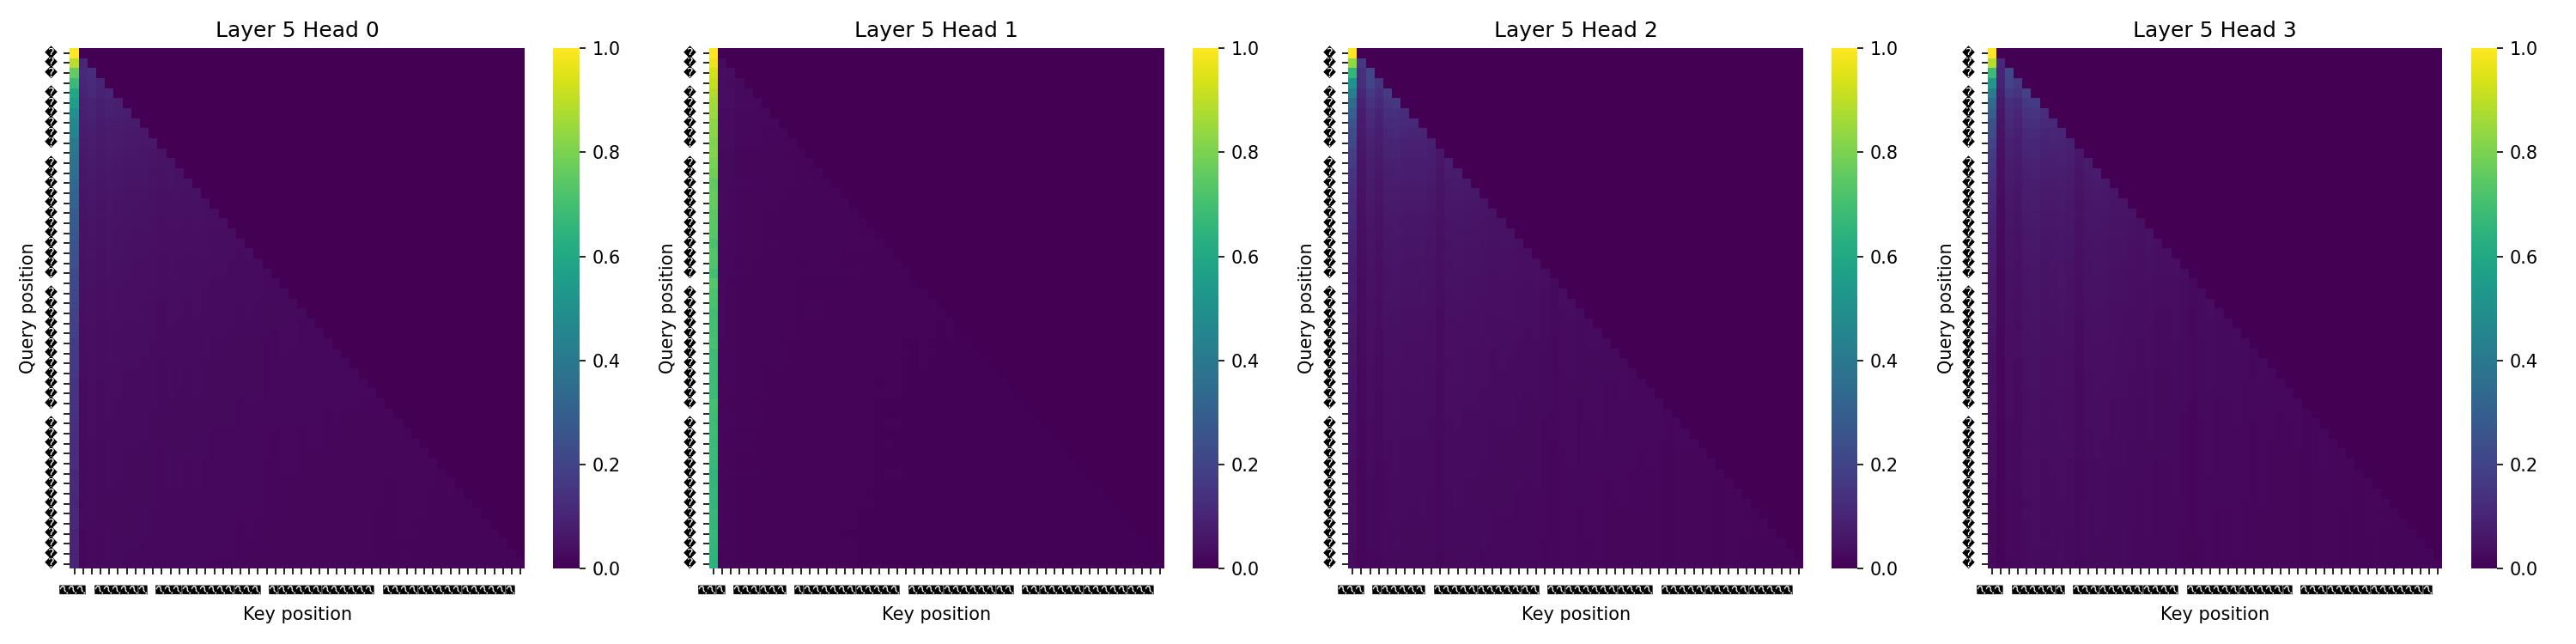
\includegraphics[width=\linewidth]{reports/nepali/attn_layer5.png}
        \caption{Layer 5 (deep).}
    \end{subfigure}
    \caption{Attention heatmaps for Nepali. They show the exact same trend as the Hindi model.}
    \label{fig:attn_nepali}
\end{figure}

\subsection{What the Layers are Doing}

\begin{enumerate}
    \item \textbf{Layer 0 (Early):} These heads mostly just look at the word immediately before them. The heatmaps show a strong diagonal line, and the mean distance is really short (about 1.5 to 2.1 tokens). They seem to just handle basic word structure.
    \item \textbf{Layer 3 (Middle):} Here, different heads start specializing. Some still look close by, but others start jumping across phrases, likely picking up on grammar rules.
    \item \textbf{Layer 5 (End):} The last layers look all over the place (high entropy) and have much longer attention distances. They are pulling context from the whole sentence to figure out what the next word should actually mean.
\end{enumerate}

\subsection{Checking the Causal Mask}

Just to be sure the model wasn't cheating, I ran a quick test in code. I changed the very last token in a sentence and checked if it altered the predictions for the earlier words. The difference was essentially zero (less than $10^{-5}$), proving that the causal mask correctly stops the model from looking into the future.

% ==============================
%   7. DISCUSSION
% ==============================
\section{Discussion}

\subsubsection*{Why did Nepali get a better perplexity score?}
Even though Nepali is supposed to be the "lower-resource" language, it scored better. I think this is because the Nepali tokenizer outputs about 28\% more bytes per token on average. Since each token packs more information, the actual sequence of tokens is "shorter" in terms of meaning, which makes predicting the next token slightly easier for the model. 

\subsubsection*{Balancing Fluency and Randomness}
If you just pick the most likely next word (greedy decoding), both models eventually get stuck repeating the same phrase over and over. From my tests, setting the temperature to 0.5 works best. It adds enough randomness to break the repetitive loops but keeps the grammar and meaning mostly intact. 

\subsubsection*{Limitations}
I trained both models for about 61K steps. They learned basic grammar, but they would probably need a lot more training time to write long, coherent paragraphs. Also, automated scores like BLEU aren't great at judging open-ended text, so human evaluation would give a much clearer picture of how good the models really are.

% ==============================
%   8. CONCLUSION
% ==============================
\section{Conclusion}

For this project, I successfully built and trained two $\approx$24M parameter language models from scratch in PyTorch for Hindi and Nepali. Both models learned well, reaching reasonable perplexities of 39.1 and 36.3. The attention maps showed that the models behave exactly like they should --- focusing locally at the start and globally at the end. When generating text, a temperature of 0.5 gave the best balance between making sense and not repeating itself. All my code, training logs, and plots are in the repo!

\end{document}
